\section{Демонстрационный пример: алгоритм двухфазной транзакции}

Протокол двухфазной транзакции (Two-Phase Commit, 2PC) представляет собой
распределённый алгоритм атомарного подтверждения, предназначенный для
координации нескольких процессов, участвующих в одной распределённой
транзакции. Его задача заключается в том, чтобы все участники либо
зафиксировали изменения (commit), либо откатили их (abort), обеспечивая
тем самым атомарность выполнения.

Протокол использует выделенный процесс-координатор (Transaction Manager, TM)
и множество участников (Resource Managers, RM). Координатор принимает
окончательное решение о результате транзакции, а участники выполняют
локальные действия и голосуют за подтверждение или отмену.

Работа протокола основана на следующих предположениях:

\begin{itemize}
    \item у каждого узла имеется стабильное хранилище (WAL);
    \item узлы могут аварийно завершаться, но не выходят из строя навсегда;
    \item записи журнала не теряются и не повреждаются при сбое;
    \item любые два узла могут обмениваться сообщениями.
\end{itemize}

В отсутствие отказов выполнение транзакции состоит из двух фаз, оно
представлено на рисунке~\ref{fig:twopc}.

\begin{figure}
  \centering
  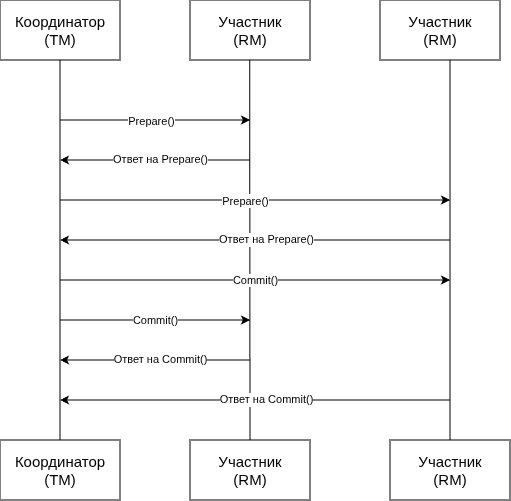
\includegraphics[scale=0.5]{inc/twopc.png}
  \caption{Двухфазный комммит}
  \label{fig:twopc}
\end{figure}

1. Фаза запроса подтверждения (voting phase).

\begin{enumerate}
    \item Координатор отправляет всем участникам сообщение
    \texttt{Prepare} (запрос на подтверждение).
    \item Каждый участник выполняет локальную часть транзакции до точки
    фиксации.
    \item Участник записывает соответствующие записи в журнал (undo/redo).
    \item Участник отправляет координатору голос:
    \begin{itemize}
        \item \texttt{Yes} (готов зафиксировать), если локальная часть
        выполнена успешно;
        \item \texttt{No} (отказ), если обнаружена ошибка.
    \end{itemize}
\end{enumerate}

2. Фаза завершения (commit phase).

\begin{itemize}
    \item Если координатор получил голос \texttt{Yes} от всех участников,
    он принимает решение \texttt{Commit}.
    \item В противном случае принимается решение \texttt{Abort}.
\end{itemize}

После принятия решения:

\begin{enumerate}
    \item Координатор рассылает сообщение \texttt{Commit} или \texttt{Abort}
    всем участникам.
    \item Каждый участник выполняет соответствующее действие:
    фиксирует изменения или откатывает их.
    \item Участник освобождает ресурсы и отправляет подтверждение
    (ACK) координатору.
    \item После получения всех подтверждений координатор завершает транзакцию.
\end{enumerate}

Протокол обеспечивает атомарность: либо все участники фиксируют изменения,
либо ни один из них не фиксирует. Однако 2PC является \emph{блокирующим}
протоколом. Если координатор выходит из строя после получения голосов
\texttt{Yes}, участники, отправившие согласие, вынуждены ожидать решения,
не имея возможности самостоятельно завершить транзакцию.

Кроме того, одновременный отказ координатора и одного из участников в фазе
завершения может привести к неопределённости состояния до восстановления
узлов. Несмотря на эти ограничения, протокол двухфазной транзакции широко
используется благодаря своей простоте и строгой атомарной семантике
\cite{bernstein2009ptp}.

\subsection{Реализация алгоритма на С}

В рамках работы был реализован прототип распределённого алгоритма
двухфазной транзакции на языке~C. Реализация состоит из двух типов
процессов: менеджер транзакции (Transaction Manager, TM) и набор
менеджеров ресурсов (Resource Manager, RM). Обмен сообщениями между
процессами вынесен в отдельный компонент сетевого взаимодействия
(\texttt{NetworkManager}) и происходит через центральный сервер сообщений (см.
\texttt{server.c} в реализации \cite{twophaseimpl}), который принимает команды
отправки и выборки сообщений и хранит их в буфере.

Логика протокола соответствует высокоуровневой модели: каждый RM выполняет
локальную работу, затем сообщает TM о готовности, а TM собирает готовности
от всех RM и после этого принимает решение о завершении транзакции
(в демонстрационном варианте --- всегда \texttt{Commit}, а \texttt{Abort} возможен
по таймауту).

\subsubsection{Менеджер ресурсов}

Основной цикл RM реализован в функции \texttt{rm\_run} (фрагмент кода приведён
на рис~\ref{fig:rm-impl}).

\begin{figure}
  \centering
  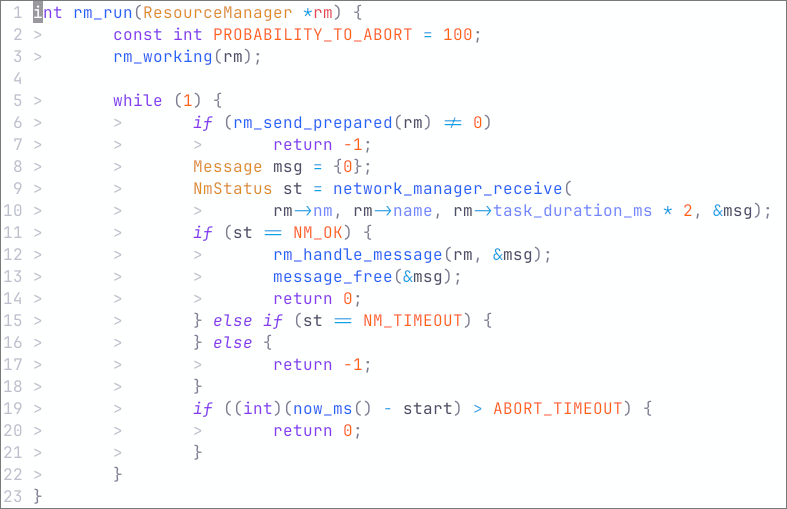
\includegraphics[scale=0.5]{inc/rm-impl.png}
  \caption{Реализация менеджера ресурсов}
  \label{fig:rm-impl}
\end{figure}

После старта процесс моделирует выполнение локальной операции
(\texttt{rm\_working}), затем переходит в фазу ожидания решения TM. Ключевой
элемент протокола --- повторная отправка сообщения о готовности при
отсутствии ответа от TM: если по истечении таймаута ответа нет, RM повторяет
отправку \texttt{Prepared}. Эта деталь важна, потому что в реальных
распределённых системах сообщения могут теряться или задерживаться, и
участникам необходимо обеспечивать прогресс протокола повторными попытками.

В реализации повторная отправка реализуется естественным образом за счёт цикла
\texttt{while (1)}: на каждой итерации RM отправляет \texttt{Prepared}, затем
вызывает \texttt{network\_manager\_receive} с конечным таймаутом. Если
результат --- \texttt{NM\_OK}, значит TM прислал решение (\texttt{Commit} или
\texttt{Abort}), и RM завершает работу после обработки сообщения. Если
результат --- \texttt{NM\_TIMEOUT}, RM не меняет состояние и переходит к
следующей итерации, тем самым повторяя отправку готовности.

Дополнительно предусмотрено аварийное завершение по общему дедлайну
(\texttt{ABORT\_TIMEOUT}): если RM слишком долго не получает решения, он
прекращает работу (в прототипе это моделирует сбой или невозможность завершить
транзакцию).

Важно отметить, что функция \texttt{rm\_send\_prepared} обновляет локальное
состояние RM: первый раз при отправке \texttt{Prepared} RM переходит в
состояние ``prepared'' и фиксирует соответствующее событие. Повторные отправки
\texttt{Prepared} не меняют состояние RM, но создают ситуации, в которых TM
может получить дубликаты сообщений.

\subsubsection{Менеджер транзакций}

Менеджер транзакций реализован в функции \texttt{tm\_run} (приведена на
рис~\ref{fig:tm-impl}). TM хранит список управляемых RM (\texttt{rm\_names}) и
множество RM, от которых уже получено \texttt{Prepared} (\texttt{prepared}).
После запуска предусмотрена инициализационная задержка
\texttt{init\_duration\_ms} --- она позволяет дать RM время отправить первые
сообщения \texttt{Prepared} прежде, чем TM начнёт интенсивно опрашивать сеть.
Эта задержка удобна для экспериментов и повторяемости, хотя не является
обязательной частью самого протокола.

\begin{figure}
  \centering
  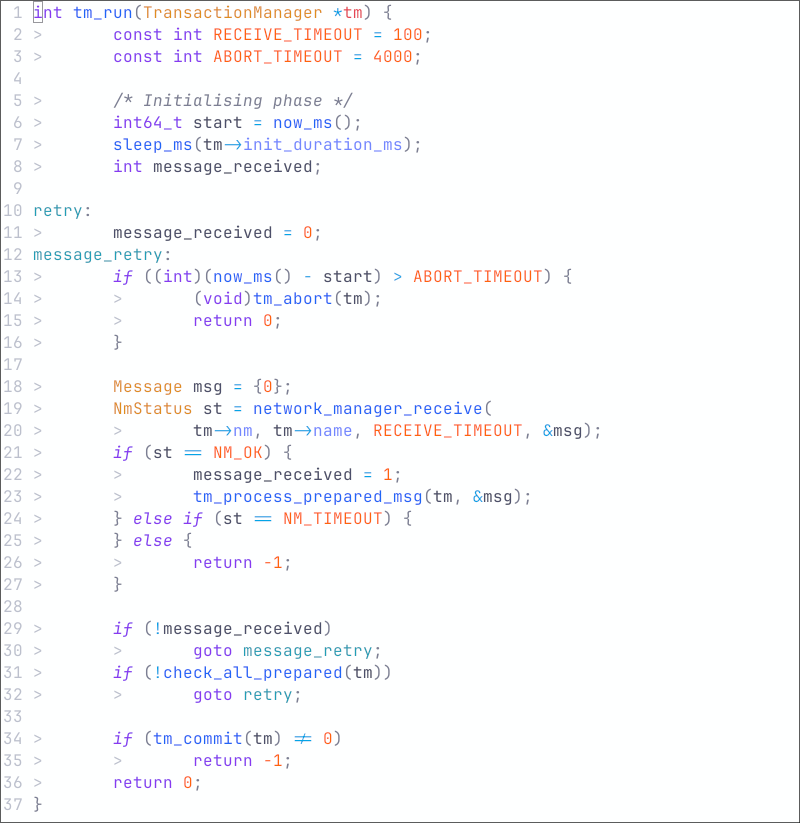
\includegraphics[scale=0.5]{inc/tm-impl.png}
  \caption{Реализация менеджера транзакций}
  \label{fig:tm-impl}
\end{figure}

Далее TM входит в цикл ожидания сообщений. Получение сообщений осуществляется
вызовом \texttt{network\_manager\_receive} с таймаутом
\texttt{RECEIVE\_TIMEOUT}. Если сообщение получено и оно содержит
\texttt{Prepared}, TM добавляет отправителя в структуру \texttt{prepared}.
После каждой успешно обработанной доставки проверяется условие завершения
подготовительной фазы: \texttt{check\_all\_prepared}. Если условие истинно, TM
рассылает всем RM сообщение \texttt{Commit} и завершает работу.

Если же сообщений долго нет и превышен общий дедлайн \texttt{ABORT\_TIMEOUT},
TM выбирает условие \texttt{Abort} и уведомляет всех участников об отмене
транзакции.

\subsection{Спецификация алгоритма на TLA+}

В качестве формальной модели используется спецификация алгоритма двухфазной
транзакции (Two-Phase Commit) на языке TLA+. Данная спецификация основана на
публичном примере из репозитория TLA+ Examples \cite{tlaexamplestwopc} и
приведена в сокращенном виде на рис.~\ref{fig:twopc-tla}.

\begin{figure}
  \centering
  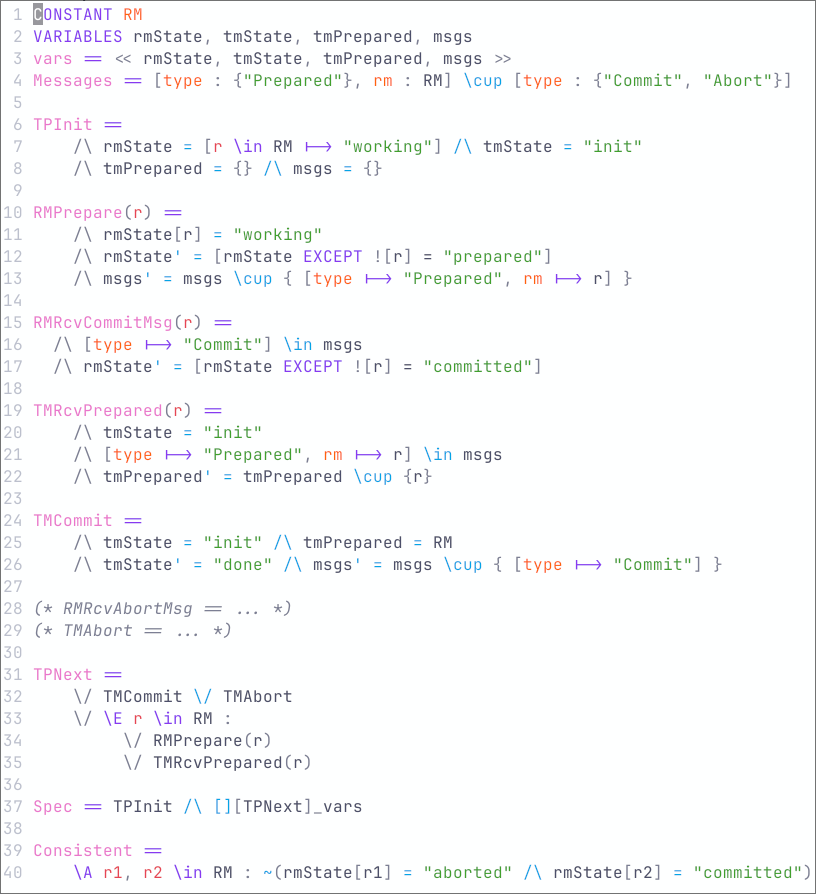
\includegraphics[scale=0.5]{inc/twopc-tla.png}
  \caption{Спецификация алгоритма двухфазной транзакции}
  \label{fig:twopc-tla}
\end{figure}

Спецификация описывает взаимодействие менеджера транзакции (TM) и множества
менеджеров ресурсов (RM), которые должны согласованно принять решение о
фиксации (commit) или откате (abort) транзакции. Менеджеры ресурсов отправляют
сообщения о готовности выполнить транзакцию, а менеджер транзакции, получив
голоса всех участников, принимает итоговое решение и рассылает соответствующее
сообщение.

Модуль сначала объявляет константу \texttt{RM}, представляющую множество
идентификаторов менеджеров ресурсов, и четыре переменные состояния:

\begin{itemize}
    \item \texttt{rmState} --- функция, отображающая каждый RM в его
    локальное управляющее состояние;
    \item \texttt{tmState} --- состояние менеджера транзакции;
    \item \texttt{tmPrepared} --- множество RM, объявивших готовность;
    \item \texttt{msgs} --- множество сообщений, отправленных в системе.
\end{itemize}

Начальное состояние задаётся предикатом \texttt{TPInit}: все RM находятся
в состоянии \texttt{"working"}, TM --- в состоянии \texttt{"init"},
а множества \texttt{tmPrepared} и \texttt{msgs} пусты.

Далее определяются действия, описывающие переходы системы.
Например, действие \texttt{RMPrepare(r)} моделирует объявление RM
с идентификатором \texttt{r} своей готовности: его состояние
изменяется на \texttt{"prepared"}, а в множество сообщений добавляется
соответствующее сообщение.

Действие \texttt{TPNext} задаёт отношение перехода системы как дизъюнкцию
всех возможных действий. Формула \texttt{Spec} объединяет начальное
условие и отношение перехода, задавая полную спецификацию поведения.

Свойства спецификации могут проверяться средствами TLC и TLAPS.
В частности, инвариант \texttt{Consistent} утверждает, что не существует
двух RM, один из которых завершил транзакцию успешно, а другой --- отменил.

Затем с помощью модуля \texttt{TraceSpec} была разработана специализированная
обёртка над спецификацией алгоритма двухфазной транзакции — модуль
\texttt{TwoPhaseTrace}. Его задача заключается в связывании конкретной
спецификации \texttt{TwoPhase} с механизмом обработки трасс: поведение
спецификации ограничивается конкретной последовательностью событий, полученной
из исполнения программы. Ее сокращенная версия представлена на
рис.~\ref{fig:twopc-spec}.

\begin{figure}
  \centering
  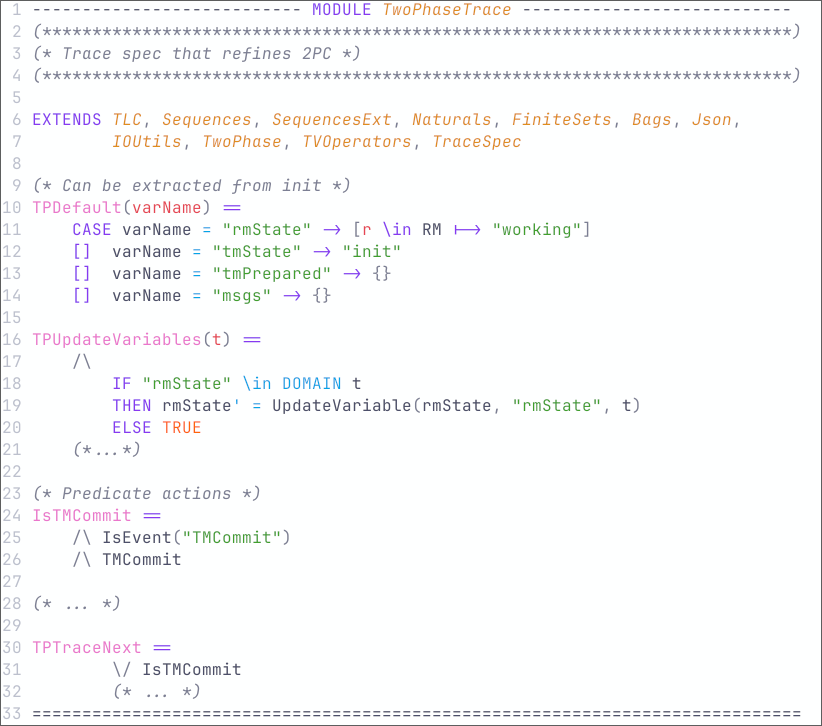
\includegraphics[scale=0.5]{inc/twopc-spec.png}
  \caption{Обертка над спецификацией алгоритма для верификации трасс}
  \label{fig:twopc-spec}
\end{figure}

\subsection{Инструментирование реализации}

После разработки реализации и спецификации алгоритма двухфазной транзакции
следующим шагом стало инструментирование этой реализации. Цель
инструментирования --- установить явное соответствие между действиями кода на
языке~C и переходами TLA+ спецификации (\texttt{RMPrepare},
\texttt{TMRcvPrepared}, \texttt{TMCommit}, \texttt{RMRcvCommitMsg} и др.).

Инструментирование выполнялось в \emph{точках линеаризации} --- местах,
где реализация завершает логически атомарный шаг протокола и обновляет
разделяемое состояние (например, изменение локального состояния RM или
добавление сообщения в множество \texttt{msgs}). В этих точках:

\begin{enumerate}
    \item регистрируются изменения переменных спецификации через
    \texttt{notify\_change};
    \item выполняется вызов \texttt{tracer\_log}, связывающий накопленные
    изменения с конкретным действием TLA+.
\end{enumerate}

\begin{figure}
  \centering
  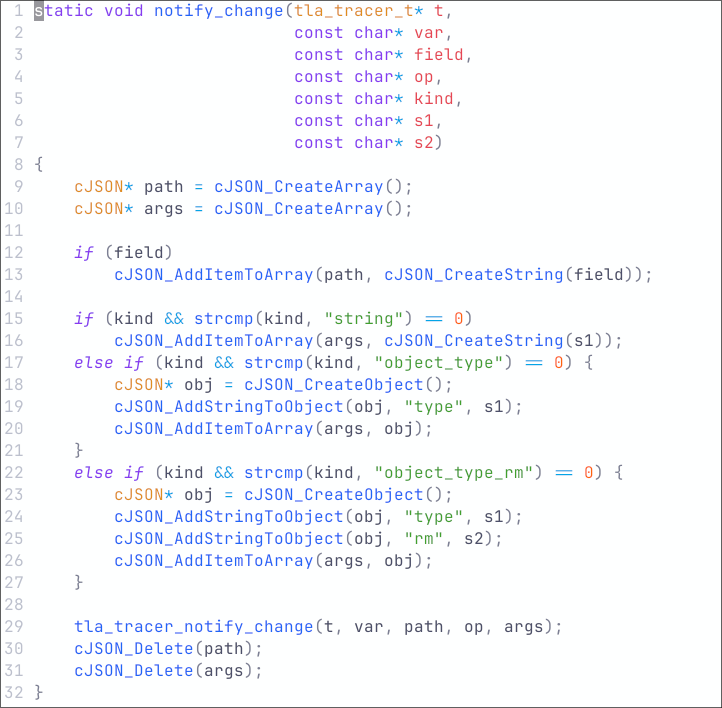
\includegraphics[scale=0.4]{inc/notify-change-impl.png}
  \caption{Вспомогательная функция для инструментирования алгоритма}
  \label{fig:notify-change}
\end{figure}

Для удобства использования библиотеки была реализована вспомогательная функция
\texttt{notify\_change}, упрощающая формирование JSON-структур \texttt{path} и
\texttt{args}. На рис~\ref{fig:notify-change} приведена сокращённая версия
функции, отражающая её логическую структуру:

Рассмотрим инструментирование отправки сообщения \texttt{Prepared}
менеджером ресурсов. В реализации эта логика сосредоточена в функции
\texttt{rm\_send\_prepared}, которая приведена на рис~\ref{fig:rm-tlac-impl}

\begin{figure}
  \centering
  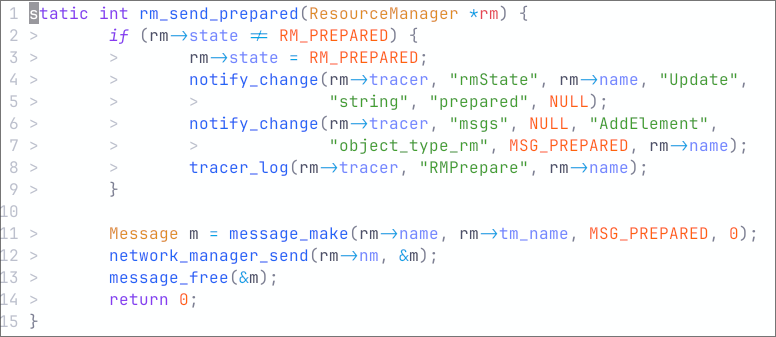
\includegraphics[scale=0.5]{inc/rm-tlac-impl.png}
  \caption{Реализация отправки сообщения prepared}
  \label{fig:rm-tlac-impl}
\end{figure}

Для RM с именем \texttt{"rm-0"} соответствующая запись трассы имеет вид,
приведенный на рис.~\ref{fig:rm-json}

\begin{figure}
  \centering
  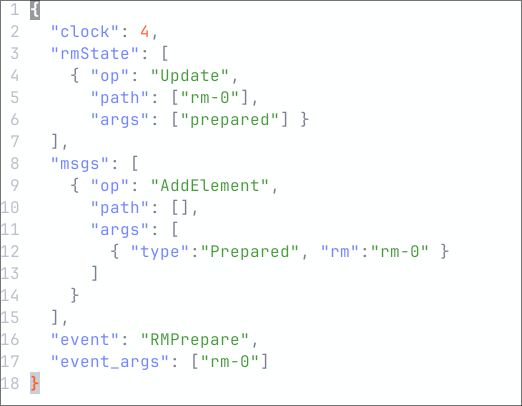
\includegraphics[scale=0.5]{inc/rm-json.png}
  \caption{Полученное сообщение трассы}
  \label{fig:rm-json}
\end{figure}

\subsection{Проверка соответствия TLA+ спецификации и исходного кода}

В процессе сопоставления реализации алгоритма двухфазной транзакции со
спецификацией на TLA+ был выявлен дефект в реализации, связанный с обработкой
сообщений \texttt{Prepared} менеджером транзакции (TM).

В корректной реализации TM должен фиксировать множество
менеджеров ресурсов, от которых получены сообщения \texttt{Prepared},
и принимать решение о фиксации транзакции только тогда, когда
\[
tmPrepared = RM,
\]
то есть когда каждый участник проголосовал за выполнение транзакции.

Однако возможна упрощённая реализация, в которой вместо множества хранится лишь
счётчик полученных сообщений \texttt{Prepared}. В этом случае условие
готовности проверяется сравнением счётчика с числом менеджеров ресурсов. Такая
реализация работает корректно, если сообщения не теряются и не дублируются.

Тем не менее, в нашей системе RM при истечении таймаута повторно отправляет
сообщение \texttt{Prepared}. Если TM не проверяет уникальность отправителя,
повторное сообщение от одного и того же RM может быть учтено несколько раз. Это
приводит к преждевременной фиксации, когда ещё не все участники объявили
готовность.

Дефект был выявлен при первом запуске \texttt{run\_pipeline\_until\_fail.sh}. В
журнале исполнения видно, что RM~\texttt{rm-0} несколько раз отправляет
сообщение \texttt{Prepared} из-за тайм-аута (см. рис.~\ref{fig:test-1}).

\begin{figure}
  \centering
  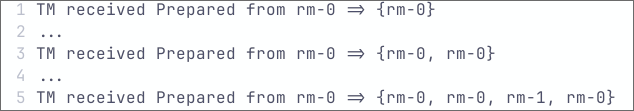
\includegraphics[scale=0.5]{inc/test-1.png}
  \caption{Повторное получение сообщения от rm-0}
  \label{fig:test-1}
\end{figure}

В результате TM принимает решение \texttt{Commit}, несмотря на то что
RM~\texttt{rm-3} ещё не отправил сообщение о готовности. Это видно из трассы:
событие \texttt{TMCommit} происходит до того, как TM получит \texttt{Prepared}
от \texttt{rm-3}. Фрагмент NDJSON-трассы приведен на рис.~\ref{fig:test-2}.

\begin{figure}
  \centering
  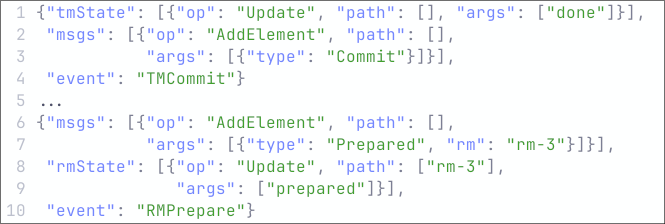
\includegraphics[scale=0.5]{inc/test-2.png}
  \caption{Часть трассы, иллюстрирующая некорректное поведение TM}
  \label{fig:test-2}
\end{figure}

То есть подтверждение транзакции произошло до получения готовности от всех RM,
что противоречит предикату \texttt{TMCommit} в спецификации.

При проверке трассы TLC ограниченная спецификация \texttt{TwoPhaseTrace} не
смогла сопоставить событие \texttt{TMCommit} с допустимым переходом исходной
модели.  Это означает, что в пространстве состояний спецификации не существует
поведения, в котором переход \texttt{TMCommit} возможен при текущем значении
переменной \texttt{tmPrepared}.

Таким образом, модельная валидация трасс позволила надёжно обнаружить
логическую ошибку реализации, которая могла бы проявляться лишь при
определённых сетевых сценариях (повторная отправка сообщений). После
исправления реализации (замена счётчика на множество уникальных RM) трассы
стали успешно проходить проверку TLC.
